\documentclass[letter]{article}

\usepackage{amsmath}
\usepackage{graphicx}
\usepackage{geometry}
\usepackage{braket} %Can do bra-ket notation with \braket{}
\usepackage{framed} %Adds the framed environment
\usepackage{fancyhdr}
\usepackage{datetime} %For formatting of header date
\usepackage{ulem} %Makes strike-through lines with \sout{}
\usepackage{booktabs} %better tables
\usepackage{multirow} %Support multi-row in tables
\usepackage[table,xcdraw]{xcolor} %Support colored rows in tables
\usdate %Month, Dth, YYYY
\geometry{
  letterpaper,
  left=1in,
  right=1in,
  bottom=1in,
  top=1in}
\pagestyle{fancy}
\lhead{NE101 Final Study Guide}
\chead{}
\rhead{}
\lfoot{}
\cfoot{\thepage}
\rfoot{\today \quad \currenttime}
\setlength\parindent{0pt}

\begin{document}
\textbf{\Large{Nuclear Engineering 101: Final Study Guide}} \\
\vspace{12pt}
%\cite[pp. 45]{krane}
%\cite[Lec 24]{lecture}

\textbf{Disclaimer:} This is not an official study guide. Stuff \sout{might}
\textbf{is} wrong. Use the lecture notes and book!
\vspace{10pt}

\textbf{Note:} Everything in this guide is from the text (Krane) or
lecture, or office hours and should be cited as completely as
possible.

\tableofcontents

\section{Reactions}

\subsection{General Information}

\begin{itemize}
\item The reaction:
  \begin{equation*}
    a + X \to Y + b
  \end{equation*}
Can be written in reaction notation as:
\begin{equation*}
  X(a,b)Y
\end{equation*}
\cite[pp. 378-379]{krane}
\item A microscopic cross section ($\sigma$) represents the ``relative
  probability for the reaction to occur.'' It can be used in the
  following equation:
  \begin{equation*}
    \begin{split}
      R= (\rho{}d)_{target}\times{}I_{beam}\times\sigma_{reaction}
    \end{split}
  \end{equation*}
Where $R$ is the reaction rate (in reactions/sec); $(\rho{}d)$ is the
density (in g/cm$^3$) times the width of the target (in cm), also
known as the areal density (put it in atoms/$cm^2$); $I_{beam}$ is the incident particle flux
(in atoms/sec); and $\sigma_{reaction}$ is the microscopic cross
section of the reaction occurring. This is only valid when very little
of the beam reacts (small $\sigma$) and everything moves in straight
lines. It can also be expressed as:
\begin{equation*}
        R= N\phi\sigma
\end{equation*}
Where $N$ is the number of target atoms, $\phi$ is the flux in
(atoms/sec/$cm^2$) and $\sigma$ is the same.~\cite[Lec. 25]{lecture}
\item Microscopic cross sections are generally given in units of
  barns. 1 barn = $10^{-24}$ cm$^2$.
  \item The cross section is not always constant over angle (it rarely
    is). So the \textit{differential cross section} is used:
    \begin{equation*}
      \frac{d\sigma}{d\Omega}
    \end{equation*}
    What is confusing, is this is just
    a number, in units of barns/steradian. It's
    representing the fact that some small number of particles
    ($d\sigma$) will strike our small detector ($d\Omega$). It is
    dependent on the angle of scatter ($\theta$) and the polraization
    of the radiation ($\phi$). Generally we assume there is no affect
    due to polarization (things are randomly polarized).

We can
    find the size of our detector $d\Omega$ in steradians, which is
    related to the area of our detector ($dA$) and the distance from
    the target ($r$) by:
    \begin{equation*}
      d\Omega = \frac{dA}{r^2}
    \end{equation*}
    Then, if we know the differential cross section at the angle of
    our detector, we can multiply to get the reaction cross section
    for our detector:
    \begin{equation*}
      \sigma_{det} = d\Omega\frac{d\sigma}{d\Omega}
    \end{equation*}
    This represents something \textbf{very specific}. This is the
    probability that incoming particles striking the target will then
    be detected by our detector. Based on the size of our detector
    ($d\Omega$) and our a priori knowledge of the number of particles
    that will be seen in a small area ($\frac{d\sigma}{d\Omega}$). The
    value of that differential cross section will probably vary with
    angle, so you have to know the differential cross section for the
    angle where your detector is to even use this. More rigorously,
    you'd integrate over the area of the detector and
    $\frac{d\sigma}{d\Omega}$ may vary over the integral:
    \begin{equation*}
      \sigma_{det} = \int_{detector}\frac{d\sigma}{d\Omega}d\Omega
    \end{equation*}
    Or, you can get the total $\sigma$ by integrating over the whole
    angle space.
\item \textbf{Rutherford Differential Scattering:} elastic Coulomb
  scattering. An incoming particle scatters off the potential of the
  target.~\cite[Lec 24]{lecture}
\item \textbf{Coulomb Excitation:} inelastic Coulomb scattering. An
  incoming particle scatters off the potential of a target and leaves
  some energy behind. This ``Coulex'' reaction can excite nuclei up
  rotational bands.~\cite[Lec. 24]{lecture}
\item Reaction $Q$-value is to create the final products at rest.
  \begin{itemize}
  \item Center of Mass Frame: products are at rest, $Q = Q$.
  \item Lab Frame: products are \textit{not} at rest. Threshold energy
    for reaction is:
    \begin{equation*}
      E_{\text{threshold}}=Q\left(\frac{m_a+m_x}{m_x}\right)
    \end{equation*}
    for a(X,Y)b.
  \end{itemize}
\item Conserved quantities in reactions:
  \begin{itemize}
  \item Total energy
  \item Linear momentum
  \item Angular momentum
  \item Parity $(-1)^l$ (except in weak interactions)
\end{itemize}
\item \textbf{Kinematics} For a reaction, $X(a,b)Y$:
  \begin{equation*}
    \begin{split}
      Q&= (m_{X}+m_{a}-m_{Y}-m_{b})c^{2}\\
      Q& =T_{Y}+T_{b}-T_{X}-T_{a}
\end{split}
\end{equation*}
\item Exothermic Q$>$0 :
  \begin{equation*}
  \begin{split}
   m_{X}+m_{a}&>m_{Y}+m_{b}\\
   T_{Y}+T_{b}&>T_{X}+T_{a}
  \end{split}
\end{equation*}
\item Endothermic Q$<$0 :
  \begin{equation*}
  \begin{split}
    m_{X}+m_{a}<&m_{Y}+m_{b}\\
T_{Y}+T_{b}<&T_{X}+T_{a}
  \end{split}
\end{equation*}
\item Reaction reaches excited states of Y:
  \begin{equation*}
Q_{ex} = (m_{X}+m_{a}-m_{Y*}-m_{b})c^{2}  = Q_{0}-E_{ex}
\end{equation*}
\item Compound nucleus:
  \begin{equation*}
Q = -T_{a} = (m_{X}+m_{a}-m_{C*})c^{2}-E_{ex}
\end{equation*}

\end{itemize}

\subsection{Photo-nuclear Interactions}

\begin{itemize}
\item A photon interacts with the nucleus directly. For this to
  happen, we need to have an energy level at the energy of the
  incoming photon.~\cite[Lec 25]{lecture}
\item There are three types of photo-nuclear interactions:
  \begin{itemize}
  \item Spontaneous emission: if the nucleus is in an energy level, it
    can release a photon to de-excite. This is an intrinsic property
    of the level.
  \item Resonant absorption: if the incoming photon is at the exact same energy
    of an energy level, it can be absorbed and the nucleus excited to
    that state. The energy of the state is the resonance energy.
  \item Stimulated emission: One photon goes in, two photons come
    out. This occurs if the incoming photon is at the resonant
    value. This is the principle by which lasers work (on the atomic
    scale), but it has not been seen for nuclei.
  \end{itemize}
  \cite[Lec 25]{lecture}
\item The cross section for this to occur ($\sigma_0$) is a function
  of the nucleus' angular momentum, and internal conversion (IC)
  factors ($\alpha$). As the probability of IC rises, photon capture
  becomes more rare, it's hard to make a nucleus capture photons when
  it wants to eject electrons.~\cite[Lec 25]{lecture}
\item The width of the emitted state:
  \begin{equation*}
    \Gamma = \frac{\hbar}{\tau}
  \end{equation*}
The longer the mean lifetime ($\tau$), the more well defined the
energy level's value is.~\cite[Lec 25]{lecture}
\end{itemize}
\subsubsection{Resonance Absorption}
\begin{itemize}
\item The resonance energy can be affected by any recoil that will
  result from the capture. This is because the nucleus needs both
  enough energy to be in its new excited state, \textbf{and} enough energy
  to recoil; so the incoming photon needs to have a little bit more
  than the expected resonance energy. As shown in
  Figure~\ref{fig:resonance_recoil}, the resonance energy has been
  shifted up by the recoil energy $E_R$ from the expected value
  $\Delta{}E$.~\cite[Lec 25]{lecture}

  \begin{figure}[hbtp]
    \centering
    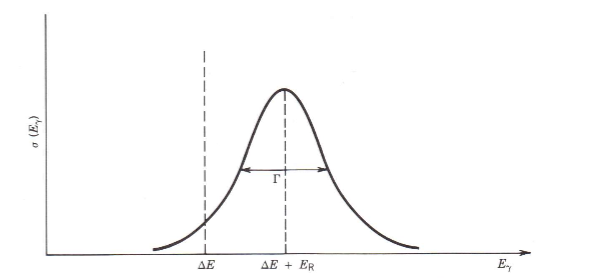
\includegraphics[scale=1.0]{images/resonance_recoil}
    \caption{Krane figure 10.23.~\cite{krane}.\label{fig:resonance_recoil}}
  \end{figure}
\item This has an exactly opposite effect on the emission
  spectrum. The absorption spectrum was shifted \textit{up} because the
  incoming photon needed extra energy to recoil the nucleus. The
  emission spectrum is shifted \textit{down} because the recoil takes some of
  the energy of the emitting photon.~\cite[Lec. 25]{lecture}
\item\textbf{Doppler broadening:} thermal motion makes the nuclei move back
  and forth, so the incoming photons energy looks doppler shifted
  either higher or lower. Therefore, a photon with energy just off the
  resonance may actually be absorbed because the relative motion can
  shift its energy to the resonance value. A wider energy range can
  now be absorbed by the resonance, so the peak gets wider or
  \textit{broadens}.~\cite[pp. 363]{krane}
\item Doppler broadening can can cause overlap between
  the emission and absorption peaks. ~\cite[Lec. 25]{lecture}
\item\textbf{Mossbauer Effect:} If a nuclei is in a crystal lattice,
  its recoil will be inhibited by the fact that \textit{its stuck in a
  lattice.} You're not just causing one nuclei to move, but
  all the ones around it, this makes the recoil energy very low, and
  therefore minimizes the shift in resonance energy by recoil. This
  allows you to nail down the \textit{actual} resonance
  energy.~\cite[Lec 25]{lecture}
\end{itemize}
\subsubsection{Giant Dipole Resonance}
\begin{itemize}
\item Ug.
\end{itemize}

\subsection{Direct Reactions}



\bibliographystyle{unsrt}
\bibliography{../NE101}
\end{document}
